\section{What representation are we converging to?}

% what is in the intersection of the multitask figure
% a good factorized world model 
% then kernels, bivariate, argument
% then say SSL related to that too

By now we hope to have convinced the reader that task and data pressures, combined with increasing model capacity, can lead to convergence. We next turn our attention to \textit{what} exactly is the endpoint of all this convergence. 

Our central hypothesis, stated in the introduction to this paper, is that the representation we are converging toward is a common statistical model of the underlying reality that generates our observations. Such a representation would naturally be useful toward many tasks (or at least toward any task grounded in reality), consistent with the multitask scaling hypothesis. Such a representation could also be relatively simple, if scientists are correct that the underlying laws of nature are indeed simple functions, consistent with the simplicity bias hypothesis.

But what exactly do we mean by ``a statistical model of the underlying reality.'' In this section, we formalize one answer in precise math. This section should be read as just one concrete candidate for the form of the Platonic representation; other candidates could be arrived at from other modeling assumptions.

\subsection{An idealized world}
We consider a world that works as follows. The world consists of a sequence of $T$ discrete events, denoted as $\mathbf{Z} \triangleq [z_1, \ldots, z_T]$, sampled from some unknown distribution $P(\mathbf{Z})$. Each event can be observed in various ways. An observation is a bijective, deterministic function $\texttt{obs}: \mathcal{Z} \rightarrow \cdot$ that maps events to an arbitrary measurement space, such as pixels, sounds, mass, force, torque, words, paragraphs, etc. 
Later in \Cref{fixme}, we discuss limitations and potential extensions to continuous and unbounded worlds, and stochastic observations, that could yield a model that better reflects real learning scenarios.
% \footnote{Extending these arguments to continuous and unbounded worlds, and stochastic observations, could yield a model that better reflects real learning scenarios.}

You can think of an event as corresponding to the state of the world at some point in time\footnote{Here we only analyze temporal sequences, but note that the same could be done with respect to events laid out in space instead.}, but it is also fine to just consider an event as any variable that indexes observations, with no further physical meaning.\footnote{We note that this latter interpretation may be more consistent with Plato's intent. Scholars have argued that his allegory of the cave rejects any notion of true world state~\cite{XX}; instead we could say that the joint distribution of indices into observations is \textit{itself} the platonic reality. The key property is that the same index $z$ maps to multiple datapoints, each a different measurement of the same underlying event.}

\subsection{Convergence via modeling cooccurrences}
In this idealized world, knowing $P(\mathbf{Z})$ would be useful for many kinds of predictions; this would constitute a world model over the events that cause our observations~\cite{XX}. 
%In this idealized world, the function $P(\mathbf{Z})$ measures the probability of some sequence of events. Knowing $P(\mathbf{Z})$ would be very useful, but estimating it is not an option since the world consists of exactly one instance of that sequence. Instead we can estimate marginals of $P(\mathbf{Z})$, which could be useful as a tractable, factorized world model. 
In the present analysis, we will restrict our attention to pairwise probabilities over events/observations. We make this simplification because our characterization of representations is only up to their kernels, which are pairwise functions over inputs. We define the \textit{cooccurrence probability}, $\mathbb{P}$, of two events $z_a$ and $z_b$ as the probability of those events both occurring within some temporal window. For simplicity, we will assume the window size is 1, so that
\begin{align}
    \mathbb{P}(z_a, z_b) \triangleq\frac{1}{2(T-1)}\sum_{t} ( & P(Z_t = z_a, Z_{t+1} = z_b) + {} \nonumber \\[-0.8ex]
    & P(Z_t = z_b, Z_{t+1} = z_a)).
\end{align}
We will argue that the Platonic representation is a model of cooccurrences of events. We leave open the question of whether representations might also be converging in terms of higher order statistics of $P(\mathbf{Z})$. 
%We articulate our precise hypothesis as follows:
%\hypbox{The Cooccurrence Kernel Hypothesis}{%
%The Platonic representation is characterized by the \textit{cooccurrence kernel}: this representation measures distance between observations as .}


%We term this model, $P(\mathbf{Z})$, where $\mathbf{Z}$ denotes a vector of events, indexed by space or time. To be precise, we consider the world as consisting of observations mediated by functions $\texttt{obs}_X$, $\texttt{obs}_Y$, and so on for modalities $X$, $Y$, etc. Each observation function maps an event (or a set of events) to a data modality. $\texttt{obs}_X(z)$ is a measurement of event $z$ in modality $X$. You can think of the $z$ as the world \textit{state}, but it is also fine to just consider each event $z$ as an \textit{index} into observations, with no further physical meaning.\footnote{We note that this latter interpretation may be more consistent with Plato's intent. Scholars have argued that his allegory of the cave rejects any notion of true world state~\cite{XX}; instead we could say that the joint distribution of indices into observations is \textit{itself} the platonic reality. The key property is that the same index $z$ maps to multiple datapoints, each a different measurement of the same underlying event.}
%By ``statistical model'' we mean a model of the joint probability of cooccurring events: how often do events $z_a$, $z_b$, $z_c$, etc occur together. By ``together'' we mean within a small window of space or time.

%How does this argument relate to our hypotheses in the previous section? The multitask scaling hypothesis (Section \ref{sec:multitask_scaling_hypothesis}) argues that representations are converging toward the small set that is effective for many tasks. $P(\mathbf{Z})$ is one such representation that has this property. In particular, $P(\mathbf{Z})$ is both 1) task-agnostic and thereby general-purpose, and 2) useful toward many tasks. The former property is because $P(\mathbf{Z})$ does not explicitly encode task -- this is an unsupervised representation. The latter property has been argued extensively in the literature: $P(\mathbf{Z})$ is a latent world model, which encodes how events unfold over space or time, and such models find use in numerous planning~\cite{XX} and reinforcement learning problems~\cite{XX}\footnote{What about actions? World models typically represent state transitions as a function of actions. In our notation, actions are just additional events in the vector $\mathbf{Z}$}. \citet{XX} argue that modeling $P(\mathbf{Z})$ (which they refer to as \textit{ZP}) is sufficient for XX.

%What about the capacity hypothesis (Section \ref{sec:capacity_hypothesis}) and the simplicity bias hypothesis (Section \ref{sec:simplicity_bias_hypothesis}? These hypotheses argue for increasing convergence as a function of model scale and priors. In this section we focus on the setting of arbitrarily large model size and unbounded data (thereby overriding the effect of any priors), so capacity and priors are not at issue. However, we note that there is a consistency between the simplicity bias and modeling $P(\mathbf{Z})$. Scientists have come up with their own $P(\mathbf{Z})$ to explain the underlying laws that govern their empirical measurements. Their $P(\mathbf{Z})$ goes by lofty names such as ``physics'', or at least ``statistical mechanics'', and they also apply strong simplicity bias, i.e. Occam's razor~\cite{XX}. Therefore, the $P(\mathbf{Z})$ that machine learning models are converging to might very well end up matching the world models scientists have theorized, and the reason here must critically depend on simplicity bias, since both real models and especially scientists have insufficient data for data constraints alone to isolate a single truth that fits the data.

% \subsection{Kernels}
% We only argue that representations are converging up to their kernels.  Kernels are bivariate functions over observations, so we argue that they reflect the pairwise statistics of $P(\mathbf{Z})$, i.e. $P(Z_a, Z_b)$ for a pair of events $\{Z_a, Z_b\}$ that occur together. We leave open the question of whether representations might also be converging in terms of higher order statistics of $P(\mathbf{Z})$.

% To provide intuition, the following statements are consistent with this general hypothesis: the distance, in representation space, between two images is proportional to the rate at which those images cooccurrence in videos; the distance between two word embeddings is proportional to the rate at which these words cooccur in sentences, and so forth.

% This part of our hypothesis is the most speculative. Like any good hypothesis, we do not aim for the precise truth, in all its gory detail, but rather an approximation to the truth that is directionally correct yet simple enough to be useful. Future work can certainly refine the arguments we give below.

% The outline of our argument is as follows:
% \begin{enumerate}
%     \item First we define a family of representation learners, in an idealized world, that result in representational convergence.
%     \item Then we argue that this world and this family of learners are reflective of real representation learning problems.
%     \item We demonstrate that these results hold in practice on a simple color modeling problem, \textcolor{red}{and also on language modeling}.
%     \item Finally we point out limitations of this model.
% \end{enumerate}

% \subsection{An idealized world}
% We consider a world that works as follows. The world consists of a sequence of events, $z_1, \ldots, z_T$. Each event can be observed in various ways. An observation is a bijective, deterministic function $\texttt{obs}: \mathcal{Z} \rightarrow \cdot$ that maps from event to an arbitrary measurement space, such as pixels, sounds, mass, force, torque, words, paragraphs, etc.\footnote{Extending these arguments to stochastic observations could yield a model that better reflects real learning scenarios.}

% You can think of an event as corresponding to the state of the world at some point in time\footnote{Here we only analyze cooccurrence in time, but note that the same could be done with respect to cooccurrences in space instead.}, but it is also fine to just consider an event as any variable that indexes observations, with no further physical meaning. Specifically, the role of events is just to define a precise notion of \textit{cooccurrence}: two observations $x$ and $y$ cooccur if and only if $x = \texttt{obs}_X(z_a)$ and $y = \texttt{obs}_Y(z_b)$ for some pair of events $z_a$ and $z_b$ within $t$ time steps of each other. Then we can define the joint probability over these observations as:
% \begin{align}
%     P_{\texttt{obs}}(x,y) %&\triangleq \frac{1}{T} \sum_{z \in \mathbf{Z}} [\texttt{cooccur}(x,y,z)]\\
%            &\triangleq \frac{1}{T} \sum_{a,b \text{ s.t. } |a-b| \leq t} [\mathds{1}(x = \texttt{obs}_X(z_a)) \nonumber \\ & \quad\quad\quad\quad\quad\text{ and } \mathds{1}(y = \texttt{obs}_Y(z_b))] \label{eqn:cooccurrence_rate_def}
% \end{align}
% We consider here a world of countably many discrete events; extensions to continuous and unbounded worlds are left to future work. The set of all events in our world is labeled as $\mathbf{Z} \triangleq \{z_1, \ldots, z_T\}$.

% For the special case where $\texttt{obs}_{X} = \texttt{obs}_{Y}$, we will denote the cooccurrence probability as $P(x_a, x_b)$. As a concrete example, $x_a$ could be a frame in a video and $x_b$ is the next frame in the video.

% Figure \ref{XX} depicts the graphical model for our idealized world.

\subsection{A family of learning algorithms that exhibit convergence to the cooccurrence kernel}
Consider an energy-based model whose objective is to model cooccurrences, in the idealized world we have defined. The model fits an energy function $E_{\theta}$ to data sampled from $\mathbb{P}_{\texttt{obs}}(x_t,x_{t+1})$, where $x_t = \texttt{obs}_X(z_t)$ and $x_{t+1}=\texttt{obs}_X(z_{t+1})$ are observations of cooccurring events $(z_t, z_{t+1})\sim \mathbb{P}$.
% $\mathbb{P}$ again denotes cooccurrence probability.%, and maximizes the log likelihood of the data under the normalized energy function.

We consider the following form for our model:
\begin{align}
    E_{\theta}(x_t,x_{t+1}) = \langle f_{\theta}(x_t), f_{\theta}(x_{t+1})) \rangle, \label{eqn:coccurrence_model}
\end{align}
%where $d$ is an arbitrary function that maps $\mathcal{X} \times \mathcal{X} \rightarrow \mathbb{R}$ (e.g., cosine distance).
%We call this a \textit{platonic learner} because, as we will next show, it converges to a platonic representation in our idealized world, in particular, a representation whose kernel is invariant to observation modality.
%Such a model could be trained with contrastive divergence~\cite{XX} or any other energy-based learning algorithm.
and optimize the maximum log-likelihood objective:
\begin{align}
    \argmin_{\theta} \mathbb{E}_{\{x_t, x_{t+1}\} \sim \mathbb{P}_{\texttt{obs}}} \Big[-\log \frac{e^{-E_{\theta}(x_t,x_{t+1})}}{Z(\theta)}\Big] \label{eqn:ML_obj}
\end{align}
where $Z$ normalizes.

Notice that any distribution $\mathbb{P}_{\texttt{obs}}$ can be represented in this way because $E_\theta$ can represent any positive semidefinite (PSD) kernel, and that $\log \mathbb{P}_\texttt{obs} + C$ is PSD for some $C$. \fixme{this is wrong} Therefore, the minimizer of \Cref{eqn:ML_obj} is:
\begin{align}
    \frac{e^{-E_{\theta}(x_t,x_{t+1})}}{Z(\theta)} = \mathbb{P}_{\texttt{obs}}(x_t,x_{t+1})
\end{align}
which implies:
\begin{align}
    \langle f_{\theta}(x_t), f_{\theta}(x_{t+1}) \rangle = -\log \mathbb{P}_{\texttt{obs}}(x_t,x_{t+1}) + C
\end{align}
for some constant $C = \log Z(\theta)$.

We will define the \textit{cooccurrence kernel} $\mathbb{K}$ as
\begin{align}
    \mathbb{K}(x_t,x_{t+1}) \triangleq -\log \mathbb{P}_{\texttt{obs}}(x_t,x_{t+1})
\end{align}
Therefore, the energy-based model we have defined is minimized by representation $f_{\theta}$ whose kernel is $\mathbb{K}$ (up to a constant offset); with sufficient data and optimization we will observe convergence to this point.

\paragraph{Invariance to observation modality}
Now consider that we have another observation modality of the same set of events, $y_t = \texttt{obs}_Y(z_t)$ and $y_{t+1} = \texttt{obs}_Y(z_{t+1})$. Our question is whether $f_Y$, trained on modality $Y$ will converge to the same kernel as $f_X$.

Recall that our idealized world consists of \textit{bijective} observation functions over discrete random variables. In this setting, we have:
\begin{align}
    \mathbb{P}_{\texttt{obs}}(x_t, x_{t+1}) = \mathbb{P}(z_t, z_{t+1})
\end{align}
and likewise for other observation variables. This is due to the fact that bijective mappings over discrete random variables preserve probability~\cite{XX}.
%from Eqn. \ref{eqn:coccurrence_model}, or from textbook probability theory~\cite{XX} (bijective mappings over discrete random variables preserve probability).

Therefore, we can rewrite the cooccurrence kernel for some observation type $X$ in terms of pairwise probabilities over $Z$:
\begin{align}
    \mathbb{K}(x_t, x_{t+1}) = -\log \mathbb{P}_{\texttt{obs}}(z_t, z_{t+1})
\end{align}
All these arguments hold not just for $X$ but also for $Y$ (or any other bijective, discrete modality), implying:
\begin{align}
    \mathbb{K}(x_t, x_{t+1}) = \mathbb{K}(y_t, y_{t+1})
\end{align}
Therefore, we observe representational convergence to a common kernel across any two modalities in our idealized world.

\subsection{Do real learners converge to the cooccurrence kernel?}

% connect analyses to pred and contr


Is this idealized setting reflective of real learning problems? 

Many representation learners do indeed model cooccurrences, in one way or another. For example, contrastive learners try to predict whether or not two observations cooccur in the same context, where, for example, the observations might be image patches and the context is an image~\cite{SimCLR}, or the observations might be sentences and the context is a paragraph~\cite{SimSCE}. Other learners work by predicting the next observation in a sequence given previous observations, aiming to model $P(x^2 | x^1)$ where $[x^1, x^2]$ is a training sequence. For these predictive learners, the cooccurrence probability, $P(x^1, x^2)$, is a sufficient statistic of the prediction problem, since $P(x^2 | x^1) = \frac{P(x^1, x^2)}{\int_{x^2} P(x^1, x^2) dx^2}$. Therefore, we conjecture that predictive objectives also lead to internal representations of cooccurrence probability\footnote{Note that $x^1$ and $x^2$ in predictive learning are \textit{not} iid, rather $x^2$ is an observation that occurs \textit{after} $x^1$}.

In Appendix \ref{sec:analysis_contrastive_predictive}, we derive kernels for a few particular constrastive and predictive learners in idealized settings. The forms of these kernels are related to $K_{\texttt{coccur}}$ but not identical to it. Thus, our mathematical analysis does not precisely claim that all representations are converging to the \textit{exact} same thing, but it does suggest that they are converging to \textit{related} things. Our \textit{hypothesis} is that 1) these related representations are roughly the same in practical settings, 2) they are similar enough that we will observe continued convergence, even if the end points are slightly different, and 3) our idealized world is close enough to reality for these claims to hold in practice.

%First we will argue that the platonic learner we have described is a kind of contrastive learner. Then we will argue that other popular learners are also benefitted from modeling $p_{\theta}(x^1,x^2)$, which suggests they may learn an internal model of the platonic kernel we have defined.

\subsection{Do these results hold in practice?}

% color
% [todo] language cpation etc.

\paragraph{Demonstration: modeling color cooccurrences}


\paragraph{\textcolor{red}{Demonstration: modeling language cooccurrences}}




% $P(x^1, x^2)$ is non-negative and symmetric.
% Does it satisfy the triangle inequality?
% $P(x^1, x^3) \leq P(x^1, x^2) + P(x^2, x^3)$


\subsection{Lossy projections}

What if the observation function is not bijective? A class label is less information than a photo, so surely the representation of class label cannot match that of a photo.

Yes, this is definitely a limitation of our hypothesis. The hypothesis requires refinement to match this setting.

We model lossiness as a blur kernel over $K_{\texttt{PMI}}$.

For each modality, we have a blur matrix $B_{X}$, $B_{Y}$, etc. The blur matrix tells us which events correspond to the same observation. 

Recall the definition of cooccurrence rate in Eqn. \ref{eqn:cooccurrence_rate_def}. We previously assumed all \texttt{obs} functions were bijective, so that, given some $x$, $\mathds{1}(x = \texttt{obs}_X(z))$ is only true for exactly one $z$. Now we will consider the case where $x$ is a \textit{partial} observation, which we formalize here to mean that $\mathds{1}(x = \texttt{obs}_X(z))$ for a set set of possible $z$'s. 

In this setting, what is the relationship between $P_X$ and $P_Z$? It is the following:
\begin{align}
    P_X(x, x^{\prime}) &= \frac{1}{T} \sum_{a,b \text{ s.t. } |a-b| \leq t} [\mathds{1}(x = \texttt{obs}_X(z_a)) \nonumber \\ & \quad\quad\quad\quad\quad\text{ and } \mathds{1}(x^{\prime} = \texttt{obs}_X(z_b))] \\
    &= \underset{\substack{
    z_a \text{ s.t. } x = \texttt{obs}_X(z_a)\\
    z_b \text{ s.t. } x^{\prime} = \texttt{obs}_X(z_b)
    }}\sum P_Z(z_a, z_b)
\end{align}

where
\begin{align}
    P_Z(z, z^{\prime}) &= \frac{1}{T} \underset{\substack{a,b \text{ s.t. }\\ |a-b| \leq t}}\sum [\mathds{1}(z = z_a) \text{ and } \mathds{1}(z^{\prime} = z_b)]
\end{align}

which implies
\begin{align}
    P_X = B^r_X (B^c_X P_Z)^T
\end{align}

We can estimate the blur kernel just like camera people do.

Here is what the estimated blur kernel looks like for text:

Across modalities, for the case where $K$ models joint probability:
\begin{align}
    P_X = B^r_X (B^c_X P_Z)^T\\
    P_Y = B^r_Y (B^c_Y P_Z)^T\\
    K_X = \log (B^r_X (B^c_X P_Z)^T)\\
    K_Y = \log (B^r_Y (B^c_Y P_Z)^T)
\end{align}
So $K_X \approx K_Y$ if the blur kernels are similar, or if they are different but the ``low frequencies'' of $P_Z$ dominate.

\subsection{Limitations to this model}

% discuss nonbijective, ctns

This is all mathematical fact in the bijective case. However, real measurements are not bijcetive. In particular, they are typically highly lossy. A strong version of our hypothesis is that this doesn't matter all that much in practice. Even though a sentence may capture different information from a photograph, their mutual information is the information that matters, and the rest is details. Or we could say that the sweet spot of the U-shaped function is at a location where different modalities agree.

In the lossy case, can we say we have $P(f(x^1), f(x^2)) = P(g(y^1), g(y^2))$ if f and g are lossy ``in the same way''? And if they are not, then a frequency argument?


%There is some time-varying state variable $z(t)$. This corresponds to the platonic reality that generates all our observations. We have no access to this variable other than through observations. An observation is some function $\texttt{obs}: \mathcal{Z} \rightarrow \cdot$ that maps from state to an arbitrary measurement space, such as pixels, sounds, mass, force, torque, words, paragraphs, etc. 

\textit{All} data is considered to be the output of some observation function, which may be arbitrarily complex. This means that even properties that we might like to call ``physics'' are here thought of just as a different set of observed measurements. If we describe a ball being thrown as having a mass $m$ and an acceleration $a$, here we interpret that as meaning that a scale will observe the value $m$ and an accelerometer will measure the acceleration as $a$. These values are \textit{not} treated as state variables. They \textit{could} be part of a model of state, but it is not necessary for our argument. State is instead considered as an abstraction with the necessary properties to generate all our observations and we are agnostic as to whether it is physicists' model of reality or something else. Indeed, scholars have intrepreted Plato's arguments as \textit{rejecting} that physical properties are any more real than other kinds of observations. Philosophy aside, however, it may be convenient to consider $z(t)$ as physical state.


Suppose we have a learner whose objective is to model the function $P(A,B)$, where $A$ is a random variable that takes on discrete values (``events'') and $B$ likewise. 

To make our argument precise, we will define what we mean by joint probability. We assume the world consists of A joint event $\{a,b\}$ 

The function $P(A,B)$ is defined as follows: if $P(A=a, B=b) = p$ then $p$ is the number of joint events where $A$ takes on the value $a$ and $B$ takes on the value $b$ divided by the total number of events.

We will further assume that our model, $p_{\theta}$ has the form:
\begin{align}
    \log p_{\theta}(A,B) \propto \langle f_{\theta}(\texttt{obs}(A)), f_{\theta}(\texttt{obs}(B)) \rangle
\end{align}
where $\texttt{obs}(\cdot)$ is some measurement function (``observation'') of the event in its argument.



%\paragraph{Conjecture: this idealized scenario relates to real representation learning scenarios}


% \paragraph{Representation learners model cooccurrence probability}

% Many representation learning algorithms are models of cooccurrence. For example, contrastive learning tries to predict whether or not two events cooccur in the same context. GPT tries to predict which event follows which. To solve these problems, it is sufficient to have a model $P(Z1,Z2)$ (this is a sufficient statistic and also easily can be transformed to the relevant predictions such as $P(Z2|Z1)$ or $P(Z1,Z2)/P(Z1)(P(Z2)$), Therefore, we conjecture that these models result in an internal representation of $P(Z1,Z2)$.

% \paragraph{Cooccurrence probability is invariant to view}
% So far we have argued that different learners all result in $P(X1, X2)$ over their domain $X$. Why should this function be the same across different domains?

% It will be if discrete RV and bijective projection $f$:
% \begin{align}
%     P(X_1, X_2) = P(f(Y_1), f(Y_2))
% \end{align}
% with $f: \mathcal{Y} \rightarrow \mathcal{X}$. Note that it doesn't matter if $X$ is physics or just a measurement. There are only measurements.


% \paragraph{Relationship to kernels}

% Encoders can be used to extract unary embeddings $f(Z1)$ and $f(Z2)$. These are what are used for further inferences or as features. We argued above that encoders represent $P(Z1,Z2)$ and we point out here that they do so via some bivariate function over embeddings:
% \begin{align}
%     g(f(z_1), f(z_2))
% \end{align}
% Often $g$ is simple, a few layers, such as in contrastive learners like SimCLR. In autoregressive models, and diffusion models, it's more complicated.

% But anyway, for all these models, there is some way to get separate embeddings for two observations, $f(z1)$ and $f(z2)$, and we have argued that the full model has learned the joint distribution $P(Z1,Z2)$.

% Therefore, we argue that there should exist some $g$ such that $g(f(z_1), f(z_2)) = P(Z1,Z2)$. This is some kernel function.

% There should exist some kernel $K$ such that $K(f(z_1), f(z_2)) = P(Z1,Z2)$. Empirically, we and others have found some kernels that work (are aligned), and our conjecture is that this is because these kernels are measuring, roughly, $P(Z1,Z2)$.




% While different models are trained in various ways, they are optimized to characterize the same underlying world. 
As we observe convergence among models, we hypothesize that different training data and tasks are simply \emph{projections} of the same underlying reality that generates what we observe (\Cref{fig:Platonic_rep}). A photo is a 2-dimensional snapshot of the world, and a text caption is a description of an event. These projections necessarily exhibit the statistical structures of the shared underlying Platonic ideal (as long as they retain rich enough information; \citet{shannon1948mathematical}). 
% For example, two events that co-occur in the real world tend to be documented together in text or photo.  
As different models are trained to better characterize such structures of respective projections, their representations become better at capturing the true statistical model of the singular reality.

\vspace{5.5pt}\textbf{Example: Convergence via modeling co-occurrences.} 
% \paragraph{Example: Convergence via modeling co-occurrences.} 
% We hypothesize that the common convergent representation is one that captures the \emph{co-occurrence} structure in the true underlying reality. 
The minimizer of common representation learning objectives gravitates towards functions defined by the co-occurrence of events. 
% Theoretical discussions and empirical observations support the notion that we are converging towards a singular, comprehensive model adept across all domains.
% 
% A central concept is that learning is driven by recognizing associations between co-occurring events. 
In particular, both contrastive and predictive learning rely on co-occurrence and are thereby optimized to recover functions of these co-occurrences. Consider a simplified universe where the true Platonic world state $\mathbf{Z}$ is observed via a bijective projection $\mathbf{X}$, each being discrete random variables. 
In this universe, perfect next-token prediction on $\mathbf{X}$ equates to modeling the probability of the next world state, given the history of previous states. This suggests that as models improve with scale and data, they inch closer to accurately representing the true joint distribution $P(\mathbf{Z}_1, \mathbf{Z}_2, \dots)$. Under such ideal conditions, models trained on any projection (\eg, modality) would be identical, adhering to the underlying distribution $P(\mathbf{Z}_1, \mathbf{Z}_2, \dots)$ of the underlying reality. 


% \begin{figure}[t]
%     \centering
%     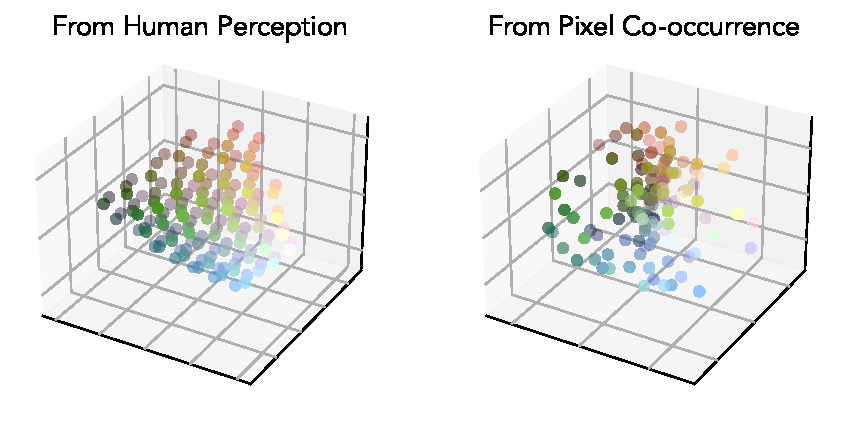
\includegraphics[width=1\linewidth]{figures/color_space.pdf}\\[-17pt]
%     % 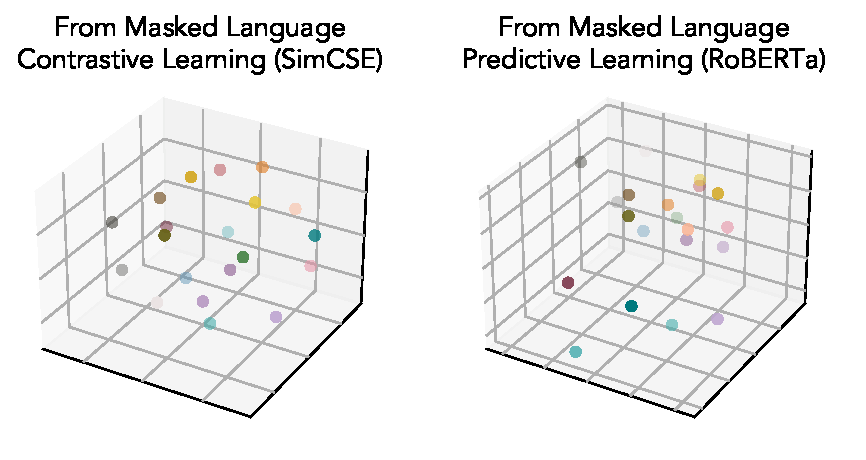
\includegraphics[width=1\linewidth]{figures/color_space_simcse_roberta.pdf}\\[-17pt]
%     \caption{\textbf{Color co-occurrence yields perceptual organization:} We optimize 3-dimensional representations of colors based on co-occurrence in CIFAR-10 images (left), and obtain a similar layout with perceptual organization from CIELAB color space (right). See Appendix \ref{sec:color_cooccurrences} for details.}
%     \label{fig:color_pAB}
% \end{figure}

This idealized analysis has its limits, especially when considering discreteness and lossy observation functions. However, similar arguments have been made theoretically and empirically \citep{zimmermann2021contrastive}. 
In particular, in the case of colors, \citet{abdou2021can} discovered that color distances in learned language representations, when trained to predict co-occurrences in \emph{text} \citep{devlin2018bert}, closely mirror human perception of these distances, which we reproduce in \Cref{fig:color_pAB}. Interestingly, they noted an increasing similarity as models scale larger and become better at modeling \emph{text} co-occurrences. In \Cref{fig:color_pAB}, we also learn representations of color based on co-occurrences in \emph{images}, and arrive at the same perceptual organization. 
Indeed, learning co-occurrence statistics in either domain recovers the \emph{same} structured representation. More generally, \citet{lu2021pretrained,mirchandani2023large} showed that models trained to autoregressively generate text also capture statistical relations in many other modalities, including symbolic reasoning, vision, protein folding, and robotics.
% We expand this analysis to visual properties beyond color.

We believe that this simple model encapsulates essential aspects of complex real-world systems, and offers a pathway towards understanding the representation that models are converging to: a unified model that is proficient across various domains and modalities, grounded in the statistical properties of the underlying world.



